\documentclass[aspectratio=169]{beamer}

%\documentclass[handout]{beamer}
%% To make 4 per page
%\usepackage{pgfpages}
%\mode<handout>{\setbeamercolor{background canvas}{bg=white}}
%\pgfpagesuselayout{4 on 1}[letterpaper,landscape]%,border shrink=5mm]

\usetheme{default}
% Slide setup, colour independent

\usepackage{amsmath,amssymb,amsthm}
\usepackage{colortbl}
\usepackage{bm}
\usepackage{xcolor}
\usepackage{dsfont}
\usepackage{setspace}
%\usepackage{subfigure}
% To use \ding{234} and the like
\usepackage{pifont}
% To cross reference between slide files
\usepackage{zref-xr,zref-user}
% Use something like
% \zexternaldocument{fileI}
% in the tex files. And cite using \zref instead of \ref

% Fields and the like
\def\IC{\mathbb{C}}
\def\IF{\mathbb{F}}
\def\II{\mathbb{I}}
\def\IJ{\mathbb{J}}
\def\IM{\mathbb{M}}
\def\IN{\mathbb{N}}
\def\IP{\mathbb{P}}
\def\IR{\mathbb{R}}
\def\IZ{\mathbb{Z}}
\def\11{\mathds{1}}


% Bold lowercase
\def\ba{\mathbf{a}}
\def\bb{\mathbf{b}}
\def\bc{\mathbf{c}}
\def\bd{\mathbf{d}}
\def\be{\mathbf{e}}
\def\bf{\mathbf{f}}
\def\bh{\mathbf{h}}
\def\bi{\mathbf{i}}
\def\bj{\mathbf{j}}
\def\bk{\mathbf{k}}
\def\bn{\mathbf{n}}
\def\bp{\mathbf{p}}
\def\br{\mathbf{r}}
\def\bs{\mathbf{s}}
\def\bu{\mathbf{u}}
\def\bv{\mathbf{v}}
\def\bw{\mathbf{w}}
\def\bx{\mathbf{x}}
\def\by{\mathbf{y}}
\def\bz{\mathbf{z}}

% Bold capitals
\def\bB{\mathbf{B}}
\def\bD{\mathbf{D}}
\def\bF{\mathbf{F}}
\def\bG{\mathbf{G}}
\def\bI{\mathbf{I}}
\def\bL{\mathbf{L}}
\def\bN{\mathbf{N}}
\def\bP{\mathbf{P}}
\def\bR{\mathbf{R}}
\def\bS{\mathbf{S}}
\def\bT{\mathbf{T}}
\def\bX{\mathbf{X}}

% Bold numbers
\def\b0{\mathbf{0}}

% Bold greek
\bmdefine{\bmu}{\bm{\mu}}
\def\bphi{\bm{\phi}}
\def\bvarphi{\bm{\varphi}}

% Bold red sentence
\def\boldred#1{{\color{red}\textbf{#1}}}
\def\defword#1{{\color{orange}\textbf{#1}}}

% Caligraphic letters
\def\A{\mathcal{A}}
\def\B{\mathcal{B}}
\def\C{\mathcal{C}}
\def\D{\mathcal{D}}
\def\E{\mathcal{E}}
\def\F{\mathcal{F}}
\def\G{\mathcal{G}}
\def\H{\mathcal{H}}
\def\I{\mathcal{I}}
\def\L{\mathcal{L}}
\def\M{\mathcal{M}}
\def\N{\mathcal{N}}
\def\P{\mathcal{P}}
\def\R{\mathcal{R}}
\def\S{\mathcal{S}}
\def\T{\mathcal{T}}
\def\U{\mathcal{U}}
\def\V{\mathcal{V}}

% tt font for code
\def\code#1{{\tt #1}}

% i.e., e.g.
\def\eg{\emph{e.g.}}
\def\ie{\emph{i.e.}}


% Operators and special symbols
\def\nbOne{{\mathchoice {\rm 1\mskip-4mu l} {\rm 1\mskip-4mu l}
{\rm 1\mskip-4.5mu l} {\rm 1\mskip-5mu l}}}
\def\cov{\ensuremath{\mathsf{cov}}}
\def\Var{\ensuremath{\mathsf{Var}\ }}
\def\Im{\textrm{Im}\;}
\def\Re{\textrm{Re}\;}
\def\det{\ensuremath{\mathsf{det}}}
\def\diag{\ensuremath{\mathsf{diag}}}
\def\nullspace{\ensuremath{\mathsf{null}}}
\def\nullity{\ensuremath{\mathsf{nullity}}}
\def\rank{\ensuremath{\mathsf{rank}}}
\def\range{\ensuremath{\mathsf{range}}}
\def\sgn{\ensuremath{\mathsf{sgn}}}
\def\Span{\ensuremath{\mathsf{span}}}
\def\tr{\ensuremath{\mathsf{tr}}}
\def\imply{$\Rightarrow$}
\def\restrictTo#1#2{\left.#1\right|_{#2}}
\newcommand{\parallelsum}{\mathbin{\!/\mkern-5mu/\!}}
\def\dsum{\mathop{\displaystyle \sum }}%
\def\dind#1#2{_{\substack{#1\\ #2}}}

\DeclareMathOperator{\GL}{GL}
\DeclareMathOperator{\Rel}{Re}
\def\Nt#1{\left|\!\left|\!\left|#1\right|\!\right|\!\right|}
\newcommand{\tripbar}{|\! |\! |}



% The beamer bullet (in base colour)
\def\bbullet{\leavevmode\usebeamertemplate{itemize item}\ }

% Theorems and the like
\newtheorem{proposition}[theorem]{Proposition}
\newtheorem{property}[theorem]{Property}
\newtheorem{importantproperty}[theorem]{Property}
\newtheorem{importanttheorem}[theorem]{Theorem}
%\newtheorem{lemma}[theorem]{Lemma}
%\newtheorem{corollary}[theorem]{Corollary}
\newtheorem{remark}[theorem]{Remark}
\setbeamertemplate{theorems}[numbered]
%\setbeamertemplate{theorems}[ams style]

%
%\usecolortheme{orchid}
%\usecolortheme{orchid}

\def\red{\color[rgb]{1,0,0}}
\def\blue{\color[rgb]{0,0,1}}
\def\green{\color[rgb]{0,1,0}}


% Get rid of navigation stuff
\setbeamertemplate{navigation symbols}{}

% Set footline/header line
\setbeamertemplate{footline}
{%
\quad p. \insertpagenumber \quad--\quad \insertsection\vskip2pt
}
% \setbeamertemplate{headline}
% {%
% \quad\insertsection\hfill p. \insertpagenumber\quad\mbox{}\vskip2pt
% }


\makeatletter
\newlength\beamerleftmargin
\setlength\beamerleftmargin{\Gm@lmargin}
\makeatother

% Colours for special pages
\def\extraContent{yellow!20}


%%%%%%%%%%%%%%%%%
\usepackage{tikz}
\usetikzlibrary{shapes,arrows}
\usetikzlibrary{positioning}
\usetikzlibrary{shapes.symbols,shapes.callouts,patterns}
\usetikzlibrary{calc,fit}
\usetikzlibrary{backgrounds}
\usetikzlibrary{decorations.pathmorphing,fit,petri}
\usetikzlibrary{automata}
\usetikzlibrary{fadings}
\usetikzlibrary{patterns,hobby}

\usetikzlibrary{backgrounds,fit,petri}


\usepackage{pgfplots}
\pgfplotsset{compat=1.6}
\pgfplotsset{ticks=none}

\usetikzlibrary{decorations.markings}
\usetikzlibrary{arrows.meta}
\tikzset{>=stealth}

% For tikz
\usetikzlibrary{shapes,arrows}
\usetikzlibrary{positioning}
\tikzstyle{cloud} = [draw, ellipse,fill=red!20, node distance=0.87cm,
minimum height=2em]
\tikzstyle{line} = [draw, -latex']


%%% For max frame images
\newenvironment{changemargin}[2]{%
\begin{list}{}{%
\setlength{\topsep}{0pt}%
\setlength{\leftmargin}{#1}%
\setlength{\rightmargin}{#2}%
\setlength{\listparindent}{\parindent}%
\setlength{\itemindent}{\parindent}%
\setlength{\parsep}{\parskip}%
}%
\item[]}{\end{list}}


% Make one image take up the entire slide content area in beamer,.:
% centered/centred full-screen image, with title:
% This uses the whole screen except for the 1cm border around it
% all. 128x96mm
\newcommand{\titledFrameImage}[2]{
\begin{frame}{#1}
%\begin{changemargin}{-1cm}{-1cm}
\begin{center}
\includegraphics[width=108mm,height=\textheight,keepaspectratio]{#2}
\end{center}
%\end{changemargin}
\end{frame}
}

% Make one image take up the entire slide content area in beamer.:
% centered/centred full-screen image, no title:
% This uses the whole screen except for the 1cm border around it
% all. 128x96mm
\newcommand{\plainFrameImage}[1]{
\begin{frame}[plain]
%\begin{changemargin}{-1cm}{-1cm}
\begin{center}
\includegraphics[width=108mm,height=76mm,keepaspectratio]{#1}
\end{center}
%\end{changemargin}
\end{frame}
}

% Make one image take up the entire slide area, including borders, in beamer.:
% centered/centred full-screen image, no title:
% This uses the entire whole screen
\newcommand{\maxFrameImage}[1]{
\begin{frame}[plain]
\begin{changemargin}{-1cm}{-1cm}
\begin{center}
\includegraphics[width=\paperwidth,height=\paperheight,keepaspectratio]
{#1}
\end{center}
\end{changemargin}
\end{frame}
}

% This uses the entire whole screen (to include in frame)
\newcommand{\maxFrameImageNoFrame}[1]{
\begin{changemargin}{-1cm}{-1cm}
\begin{center}
\includegraphics[width=\paperwidth,height=0.99\paperheight,keepaspectratio]
{#1}
\end{center}
\end{changemargin}
}

% Make one image take up the entire slide area, including borders, in beamer.:
% centered/centred full-screen image, no title:
% This uses the entire whole screen
\newcommand{\maxFrameImageColor}[2]{
\begin{frame}[plain]
\setbeamercolor{normal text}{bg=#2!20}
\begin{changemargin}{-1cm}{-1cm}
\begin{center}
\includegraphics[width=\paperwidth,height=\paperheight,keepaspectratio]
{#1}
\end{center}
\end{changemargin}
\end{frame}
}


\usepackage{tikz}
\usetikzlibrary{patterns,hobby}
\usepackage{pgfplots}
\pgfplotsset{compat=1.6}
\pgfplotsset{ticks=none}

\usetikzlibrary{backgrounds}
\usetikzlibrary{decorations.markings}
\usetikzlibrary{arrows.meta}
\tikzset{>=stealth}

\tikzset{
  clockwise arrows/.style={
    postaction={
      decorate,
      decoration={
        markings,
        mark=between positions 0.1 and 0.9 step 40pt with {\arrow{>}},
   }}}}


   %%%%%%%%%%%
% To have links to parts in the outline
\makeatletter
\AtBeginPart{%
  \addtocontents{toc}{\protect\beamer@partintoc{\the\c@part}{\beamer@partnameshort}{\the\c@page}}%
}
%% number, shortname, page.
\providecommand\beamer@partintoc[3]{%
  \ifnum\c@tocdepth=-1\relax
    % requesting onlyparts.
    \makebox[6em]{Part #1:} \textcolor{green!30!blue}{\hyperlink{#2}{#2}}
    \par
  \fi
}
\define@key{beamertoc}{onlyparts}[]{%
  \c@tocdepth=-1\relax
}
\makeatother%

\newcommand{\nameofthepart}{}
\newcommand{\nupart}[1]%
    {   \part{#1}%
        \renewcommand{\nameofthepart}{#1}%
        {
          \setbeamercolor{background canvas}{bg=orange!50}
          \begin{frame}{#1}%\partpage 
          \hypertarget{\nameofthepart}{}\tableofcontents%
          \end{frame}
        }
    }



\usecolortheme{orchid}

%% Listings
\usepackage{listings}
\definecolor{mygreen}{rgb}{0,0.6,0}
\definecolor{mygray}{rgb}{0.5,0.5,0.5}
\definecolor{mymauve}{rgb}{0.58,0,0.82}
\definecolor{mygold}{rgb}{1,0.843,0}
\definecolor{myblue}{rgb}{0.537,0.812,0.941}

\definecolor{lgreen}{rgb}{0.6,0.9,.6}
\definecolor{lred}{rgb}{1,0.5,.5}

\lstloadlanguages{R}
\lstset{ %
  language=R,
  backgroundcolor=\color{black!05},   % choose the background color
  basicstyle=\footnotesize\ttfamily,        % size of fonts used for the code
  breaklines=true,                 % automatic line breaking only at whitespace
  captionpos=b,                    % sets the caption-position to bottom
  commentstyle=\color{mygreen},    % comment style
  escapeinside={\%*}{*)},          % if you want to add LaTeX within your code
  keywordstyle=\color{red},       % keyword style
  stringstyle=\color{mygold},     % string literal style
  keepspaces=true,
  columns=fullflexible,
  tabsize=4,
}
% Could also do (in lstset)
% basicstyle==\fontfamily{pcr}\footnotesize
\lstdefinelanguage{Renhanced}%
  {keywords={abbreviate,abline,abs,acos,acosh,action,add1,add,%
      aggregate,alias,Alias,alist,all,anova,any,aov,aperm,append,apply,%
      approx,approxfun,apropos,Arg,args,array,arrows,as,asin,asinh,%
      atan,atan2,atanh,attach,attr,attributes,autoload,autoloader,ave,%
      axis,backsolve,barplot,basename,besselI,besselJ,besselK,besselY,%
      beta,binomial,body,box,boxplot,break,browser,bug,builtins,bxp,by,%
      c,C,call,Call,case,cat,category,cbind,ceiling,character,char,%
      charmatch,check,chol,chol2inv,choose,chull,class,close,cm,codes,%
      coef,coefficients,co,col,colnames,colors,colours,commandArgs,%
      comment,complete,complex,conflicts,Conj,contents,contour,%
      contrasts,contr,control,helmert,contrib,convolve,cooks,coords,%
      distance,coplot,cor,cos,cosh,count,fields,cov,covratio,wt,CRAN,%
      create,crossprod,cummax,cummin,cumprod,cumsum,curve,cut,cycle,D,%
      data,dataentry,date,dbeta,dbinom,dcauchy,dchisq,de,debug,%
      debugger,Defunct,default,delay,delete,deltat,demo,de,density,%
      deparse,dependencies,Deprecated,deriv,description,detach,%
      dev2bitmap,dev,cur,deviance,off,prev,,dexp,df,dfbetas,dffits,%
      dgamma,dgeom,dget,dhyper,diag,diff,digamma,dim,dimnames,dir,%
      dirname,dlnorm,dlogis,dnbinom,dnchisq,dnorm,do,dotplot,double,%
      download,dpois,dput,drop,drop1,dsignrank,dt,dummy,dump,dunif,%
      duplicated,dweibull,dwilcox,dyn,edit,eff,effects,eigen,else,%
      emacs,end,environment,env,erase,eval,equal,evalq,example,exists,%
      exit,exp,expand,expression,External,extract,extractAIC,factor,%
      fail,family,fft,file,filled,find,fitted,fivenum,fix,floor,for,%
      For,formals,format,formatC,formula,Fortran,forwardsolve,frame,%
      frequency,ftable,ftable2table,function,gamma,Gamma,gammaCody,%
      gaussian,gc,gcinfo,gctorture,get,getenv,geterrmessage,getOption,%
      getwd,gl,glm,globalenv,gnome,GNOME,graphics,gray,grep,grey,grid,%
      gsub,hasTsp,hat,heat,help,hist,home,hsv,httpclient,I,identify,if,%
      ifelse,Im,image,\%in\%,index,influence,measures,inherits,install,%
      installed,integer,interaction,interactive,Internal,intersect,%
      inverse,invisible,IQR,is,jitter,kappa,kronecker,labels,lapply,%
      layout,lbeta,lchoose,lcm,legend,length,levels,lgamma,library,%
      licence,license,lines,list,lm,load,local,locator,log,log10,log1p,%
      log2,logical,loglin,lower,lowess,ls,lsfit,lsf,ls,machine,Machine,%
      mad,mahalanobis,make,link,margin,match,Math,matlines,mat,matplot,%
      matpoints,matrix,max,mean,median,memory,menu,merge,methods,min,%
      missing,Mod,mode,model,response,mosaicplot,mtext,mvfft,na,nan,%
      names,omit,nargs,nchar,ncol,NCOL,new,next,NextMethod,nextn,%
      nlevels,nlm,noquote,NotYetImplemented,NotYetUsed,nrow,NROW,null,%
      numeric,\%o\%,objects,offset,old,on,Ops,optim,optimise,optimize,%
      options,or,order,ordered,outer,package,packages,page,pairlist,%
      pairs,palette,panel,par,parent,parse,paste,path,pbeta,pbinom,%
      pcauchy,pchisq,pentagamma,persp,pexp,pf,pgamma,pgeom,phyper,pico,%
      pictex,piechart,Platform,plnorm,plogis,plot,pmatch,pmax,pmin,%
      pnbinom,pnchisq,pnorm,points,poisson,poly,polygon,polyroot,pos,%
      postscript,power,ppoints,ppois,predict,preplot,pretty,Primitive,%
      print,prmatrix,proc,prod,profile,proj,prompt,prop,provide,%
      psignrank,ps,pt,ptukey,punif,pweibull,pwilcox,q,qbeta,qbinom,%
      qcauchy,qchisq,qexp,qf,qgamma,qgeom,qhyper,qlnorm,qlogis,qnbinom,%
      qnchisq,qnorm,qpois,qqline,qqnorm,qqplot,qr,Q,qty,qy,qsignrank,%
      qt,qtukey,quantile,quasi,quit,qunif,quote,qweibull,qwilcox,%
      rainbow,range,rank,rbeta,rbind,rbinom,rcauchy,rchisq,Re,read,csv,%
      csv2,fwf,readline,socket,real,Recall,rect,reformulate,regexpr,%
      relevel,remove,rep,repeat,replace,replications,report,require,%
      resid,residuals,restart,return,rev,rexp,rf,rgamma,rgb,rgeom,R,%
      rhyper,rle,rlnorm,rlogis,rm,rnbinom,RNGkind,rnorm,round,row,%
      rownames,rowsum,rpois,rsignrank,rstandard,rstudent,rt,rug,runif,%
      rweibull,rwilcox,sample,sapply,save,scale,scan,scan,screen,sd,se,%
      search,searchpaths,segments,seq,sequence,setdiff,setequal,set,%
      setwd,show,sign,signif,sin,single,sinh,sink,solve,sort,source,%
      spline,splinefun,split,sqrt,stars,start,stat,stem,step,stop,%
      storage,strstrheight,stripplot,strsplit,structure,strwidth,sub,%
      subset,substitute,substr,substring,sum,summary,sunflowerplot,svd,%
      sweep,switch,symbol,symbols,symnum,sys,status,system,t,table,%
      tabulate,tan,tanh,tapply,tempfile,terms,terrain,tetragamma,text,%
      time,title,topo,trace,traceback,transform,tri,trigamma,trunc,try,%
      ts,tsp,typeof,unclass,undebug,undoc,union,unique,uniroot,unix,%
      unlink,unlist,unname,untrace,update,upper,url,UseMethod,var,%
      variable,vector,Version,vi,warning,warnings,weighted,weights,%
      which,while,window,write,\%x\%,x11,X11,xedit,xemacs,xinch,xor,%
      xpdrows,xy,xyinch,yinch,zapsmall,zip},%
   otherkeywords={!,!=,~,$,*,\%,\&,\%/\%,\%*\%,\%\%,<-,<<-,_,/},%
   alsoother={._$},%
   sensitive,%
   morecomment=[l]\#,%
   morestring=[d]",%
   morestring=[d]'% 2001 Robert Denham
  }%

%%%%%%% 
%% Definitions in yellow boxes
\usepackage{etoolbox}
\setbeamercolor{block title}{use=structure,fg=structure.fg,bg=structure.fg!40!bg}
\setbeamercolor{block body}{parent=normal text,use=block title,bg=block title.bg!20!bg}

\BeforeBeginEnvironment{definition}{%
	\setbeamercolor{block title}{fg=black,bg=yellow!20!white}
	\setbeamercolor{block body}{fg=black, bg=yellow!05!white}
}
\AfterEndEnvironment{definition}{
	\setbeamercolor{block title}{use=structure,fg=structure.fg,bg=structure.fg!20!bg}
	\setbeamercolor{block body}{parent=normal text,use=block title,bg=block title.bg!50!bg, fg=black}
}
\BeforeBeginEnvironment{importanttheorem}{%
	\setbeamercolor{block title}{fg=black,bg=red!20!white}
	\setbeamercolor{block body}{fg=black, bg=red!05!white}
}
\AfterEndEnvironment{importanttheorem}{
	\setbeamercolor{block title}{use=structure,fg=structure.fg,bg=structure.fg!20!bg}
	\setbeamercolor{block body}{parent=normal text,use=block title,bg=block title.bg!50!bg, fg=black}
}
\BeforeBeginEnvironment{importantproperty}{%
	\setbeamercolor{block title}{fg=black,bg=red!50!white}
	\setbeamercolor{block body}{fg=black, bg=red!30!white}
}
\AfterEndEnvironment{importantproperty}{
	\setbeamercolor{block title}{use=structure,fg=structure.fg,bg=structure.fg!20!bg}
	\setbeamercolor{block body}{parent=normal text,use=block title,bg=block title.bg!50!bg, fg=black}
}


% Beginning of a section
\AtBeginSection[]{
	{
		\setbeamercolor{background canvas}{bg=yellow!10}
		\begin{frame}[noframenumbering,plain]
			\framesubtitle{\nameofthepart Chapter \insertromanpartnumber \ -- \iteminsert{\insertpart}}
			\tableofcontents[
				currentsection,
				sectionstyle=show/shaded,
				subsectionstyle=show/show/hide]
		\end{frame}
	\addtocounter{page}{-1}
	%\addtocounter{framenumber}{-1} 
	}
}

% Beginning of a section
\AtBeginSubsection[]{
	{
		\setbeamercolor{background canvas}{bg=green!10}
		\begin{frame}[noframenumbering,plain]
				\framesubtitle{\nameofthepart Chapter \insertromanpartnumber \ -- \iteminsert{\insertpart}}
				\tableofcontents[
					currentsection,
					sectionstyle=show/show,
					currentsubsection,
					subsectionstyle=show/shaded/hide]
			\end{frame}
		\addtocounter{page}{-1}
	}
}


% To have theorems and everything derived prefixed by the slide set
% number
\renewcommand{\thetheorem}{3.\arabic{theorem}}



\title{Eigenvalues, eigenvectors, similarity and Ger\v{s}gorin disks}
\author{Julien Arino}
\date{Fall 2023}

%%%%%%%%%%%%%%%%%%%%%
%%%%%%%%%%%%%%%%%%%%%
%%%%%%%%%%%%%%%%%%%%%
%%%%%%%%%%%%%%%%%%%%%
%%%%%%%%%%%%%%%%%%%%%
%%%%%%%%%%%%%%%%%%%%%
%%%%%%%%%%%%%%%%%%%%%
%%%%%%%%%%%%%%%%%%%%%
\begin{document}

% The title page
\begin{frame}[noframenumbering,plain]
  \begin{tikzpicture}[remember picture,overlay]
    \node[above right,inner sep=0pt] at (current page.south west)
    {
        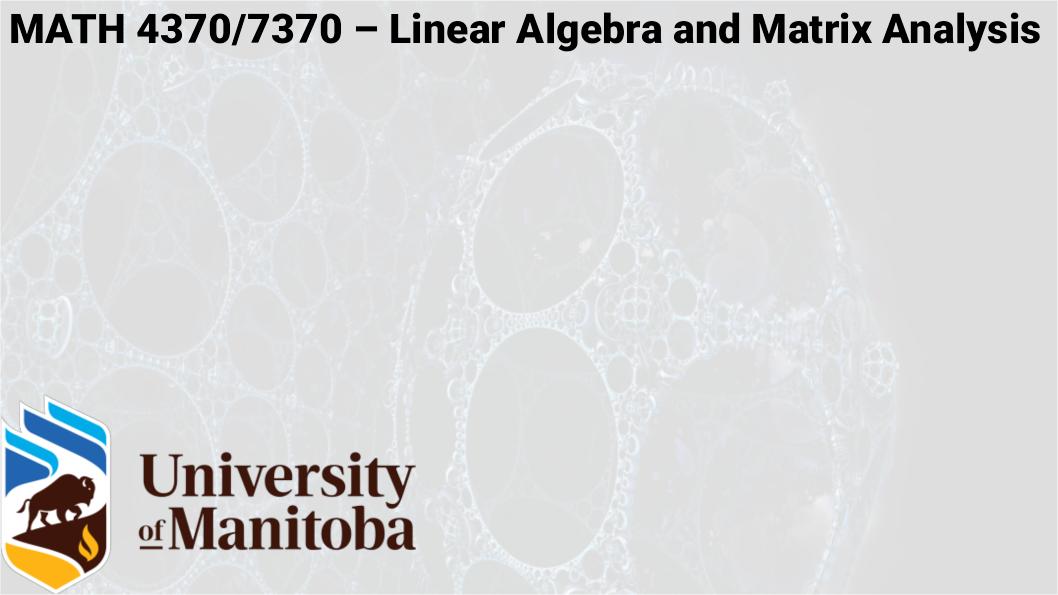
\includegraphics[width=\paperwidth]{title-page-picture.png}
    };
\end{tikzpicture}
	\titlepage
\end{frame}
\addtocounter{page}{-1}
  
  
\begin{frame}{Outline}
	  \tableofcontents[hideallsubsections]
\end{frame}
\addtocounter{page}{-1}


%%%%%%%%%%%%%%%%%%%%%%%%%%%
%%%%%%%%%%%%%%%%%%%%%%%%%%%
%%%%%%%%%%%%%%%%%%%%%%%%%%%
%%%%%%%%%%%%%%%%%%%%%%%%%%%
\section{Eigenpairs}


\begin{frame}
\begin{definition}\label{def:eigenvalue}
Let $A\in \mathcal{M}_{n}(\IF)$. If $\lambda\in \IC$ and $\bv\neq\b0\in \IF^n$ are such that $A\bv=\lambda\bv$, then $\lambda$ is an \defword{eigenvalue} of $A$ associated to the \defword{eigenvector} $\bv$. We also say that $(\lambda, \bv)$ form an \defword{eigenpair}.
\end{definition}
\end{frame}


\begin{frame}
The eigenpair equation takes the form $A\bv= \lambda\bv$, for $\bv\neq\b0$. Rewriting this,
\[
A\bv=\lambda\bv \iff A\bv-\lambda\bv = \b0 \iff A\bv-\lambda\II\bv=\b0\iff (A-\lambda \II)\bv=\b0
\]
(We could also have obtained $(\lambda\II-A)\bv=\b0$)
\vfill
Hence, since we seek $\bv\neq\b0$, the homogeneous system $(A-\lambda\II)\bv=\b0$ must have non-trivial solutions; this implies that $A-\lambda\II$ must be \emph{singular}. So, if $\lambda$ is an eigenvalue, there must hold that $\det(A-\lambda\II)=0$ 
\vfill
\begin{remark}
It is essential to remember that one seeks a \emph{nonzero} vector $\bv$. Clearly, if $\bv=\b0$, then $A\bv=\lambda\bv$ for any $\lambda$, since this just means that $\b0=\b0$
\end{remark}
\end{frame}

\begin{frame}
Often, we use normalised eigenvectors, $\tilde\bv=\bv/||\bv||$, so that $\|\tilde\bv\|=1$
\vfill
Also, for eigenvectors $\bv$ that have all their components nonpositive, we typically use $-\bv$, so that all components are nonnegative.
\end{frame}


\begin{frame}
\begin{definition}[Spectrum of a matrix]
  The \defword{spectrum} of $A\in \mathcal{M}_n$ is the set of all its eigenvalues and its denoted $\sigma(A)$
\end{definition}
\vfill
\begin{theorem}
$0\in \sigma(A)\iff A$ is singular
\end{theorem}
\vfill
\begin{theorem}\label{th:spectrum_shift}
$A\in \mathcal{M}_{n}(\IF)$, $\lambda, \mu \in \IC$ given. Then 
$\lambda\in \sigma(A)$ if and only if $\lambda+\mu \in \sigma(A+\mu\II)$
\end{theorem}
\end{frame}


%%%%%%%%%%%%%%%%%%%%%%%%
%%%%%%%%%%%%%%%%%%%%%%%%
%%%%%%%%%%%%%%%%%%%%%%%%
%%%%%%%%%%%%%%%%%%%%%%%%
\section{Characteristic equation and algebraic multiplicity}

\begin{frame}
\begin{definition}[Characteristic polynomial/equation]
The \defword{characteristic polynomial} of $A\in \mathcal{M}_n$ is 
\[p_A(z)= \det(A-z\II).\]
The \defword{characteristic equation} of $A$ is $p_A(z)=0$
\end{definition}
\vfill
By the Fundamental Theorem of Algebra, if $p_A(z)$ has degree $n$, then $p_A(z)$ has $n$ complex roots including multiplicity (or at most $n$ roots if not counting multiplicity)
\vfill
These roots are the eigenvalues of $A$ and thus $\sigma(A)$ has at most $n$ elements in $\IC$
\end{frame}


\begin{frame}
\begin{theorem}
Let $A\in \mathcal{M}_n$. Then 
\[
\tr(A)= \sum\limits_{i=1}^n \lambda_i 
\quad\textrm{and}\quad 
\det(A)= \prod\limits_{i=1}^n \lambda_i
\]
\end{theorem}   
\end{frame}

\begin{frame}
\begin{theorem}
Let $p(T)$ be a $k$-degree polynomial. If $(\lambda,\bv)$ eigenpair of $A\in \mathcal{M}_n$, then $(p(\lambda),\bv)$ is an eigenpair for $p(A)$
\end{theorem}
\vfill
\begin{definition}[Algebraic multiplicity of an eigenvalue]
Let $A\in \mathcal{M}_{n}$. The (\defword{algebraic}) \defword{multiplicity} of $\lambda\in \sigma(A)$ is its multiplicity as a zero of the characteristic polynomial $p_A(\lambda)$
\end{definition}    
\end{frame}

\begin{frame}
\begin{definition}[Spectral radius of a matrix]
The \defword{spectral radius} of $A\in \mathcal{M}_n$ is 
\[
  \rho(A)= \max \{ | \lambda |, \mid \lambda\in \sigma(A)\}
\]
\end{definition}
\vfill
\begin{proposition}
For all $\lambda\in \sigma(A)$, $A\in \mathcal{M}_n$, $\lambda$ lies in the closed bounded disk in $\IC$, 
\[
  \{ z\in \IC: z| \leq \rho(A)\}
\]
\end{proposition}
\vfill
\begin{theorem}[Every square matrix is close to nonsingular matrices]
Let $A\in \mathcal{M}_n$, then there exists $\delta>0$ such that $A+\varepsilon\II$ is non-singular for $0< | \varepsilon | <\delta$
\end{theorem}
\end{frame}

\begin{frame}
\begin{theorem}
Let $A\in \mathcal{M}_{n}$. 
Suppose that $\lambda\in \sigma(A)$ has algebraic multiplicity $k$. 
Then 
\[
  \rank (A-\lambda\II)\geq n-k
\]
with equality when $k=1$
\end{theorem}
\end{frame}

%%%%%%%%%%%%%%%%%%%%%%%%
%%%%%%%%%%%%%%%%%%%%%%%%
%%%%%%%%%%%%%%%%%%%%%%%%
%%%%%%%%%%%%%%%%%%%%%%%%
\section{Similarity}

\begin{frame}
\begin{definition}[Similarity/permutation similarity]
Let $A,\, B\in\mathcal{M}_n$. We say that $B$ is \defword{similar} to $A$ if there exists a nonsingular $S\in \mathcal{M}_n$ such that 
\[
  B=S^{-1} AS
\]
The transformation $A\mapsto S^{-1}AS$ is a \defword{similarity transformation} with similarity matrix $S$. 
If $S=P$ with $P$ a \defword{permutation matrix} and that $B= P^{T} AP$, $A$ and $B$ are \defword{permutation similar}. 
In both cases, we denote ``$A$ similar to $B$'' as $A \sim B$
\end{definition}
\vfill
\begin{theorem}
Similarity is an equivalence relation, i.e., it is reflexive, symmetric, and transitive
\end{theorem}
\end{frame}

\begin{frame}
\begin{theorem}
 Let $A, \, B\in \mathcal{M}_n$. If $A$ is similar to $B$, then they have the same characteristic polynomial, \ie,
 \[p_A(t)= p_B(t) 
\]
\end{theorem}
\vfill
\begin{corollary}
Let $A,\, B\in \mathcal{M}_n$. If $A\sim B$, then 
\begin{enumerate}
\item $A$ and $B$ have the same eigenvalues
\item If $B$ is a diagonal matrix, then the main diagonal entries are the eigenvalues of $A$
\item $B=0\iff A=0$
\item $B=\II\iff A=\II$
\end{enumerate}
\end{corollary}
\end{frame}

\begin{frame}
\begin{definition}
If $A\in \mathcal{M}_n$. If $A$ is similar to a diagonal matrix, then $A$ is \defword{diagonalisable}
\end{definition}
\end{frame}

\begin{frame}
\begin{theorem}
Let $A\in \mathcal{M}_n$. 
\begin{enumerate}
\item 
\begin{equation}
A\sim \begin{pmatrix}
\Lambda & C\\
0& D
\end{pmatrix}
\end{equation}
with $\Lambda= diag(\lambda_1,\ldots, \lambda_k)$, $D\in \mathcal{M}_{n-k}$, $1\leq k\leq n$ $\iff$ $k$ linear independent vectors in $\IC^n$, each of which is an eigenvector of $A$
\item $A$ diagonalisable $\iff$ there are $n$ linearly independent eigenvectors of $A$
\end{enumerate}
\end{theorem}
\end{frame}

\begin{frame}
\addtocounter{theorem}{-1}
\begin{theorem}[continued]
\begin{enumerate}
\setcounter{enumi}{2}
\item If $x^{(1)},\ldots, x^{(n)}$ are linear independent eigenvectors of $A$, define 
\[S= [ x^{(1)} \ldots x^{(n)}].\]
Then $S^{-1} AS$ is diagonal.
\item If 
\[A\sim \begin{pmatrix}
\Lambda & C\\
0& D
\end{pmatrix},\]
then the diagonal entries of $\Lambda$ are eigenvalues of $A$, if $A\sim\Lambda = \diag (\lambda_1, \ldots, \lambda_n)$, then $\lambda_1, \ldots, \lambda_n$ are the eigenvalues of $A$
\end{enumerate}
\end{theorem}
\end{frame}


\begin{frame}
\begin{lemma}
Let $\lambda_1, \ldots, \lambda_k$, $k \geq 2$ be $k$ distinct eigenvalue of $A$. Let $x^{(i)}$ be an eigenvector associated to $\lambda_i$, $i= 1, \ldots, k$. Then $x^{(1)}, \ldots, x^{(k)}$ are linear independent
\end{lemma}
\vfill
\begin{theorem}
If $A\in \mathcal{M}_n$ has $n$ distinct eigenvalues, then it is diagonalisable
\end{theorem}
\vfill
\begin{lemma}
Let $B= \bigoplus\limits_{i=1}^d B_{ii}$. Then $B$ is diagonalisable if and only if each of the $B_{ii}$ is diagonalisable
\end{lemma}
\end{frame}


\begin{frame}
\begin{definition}
Two matrices $A$ and $B$ in $\mathcal{M}_n$ are \defword{simultaneously diagonalisable} if there exists a matrix $S\in \mathcal{M}_n$ non-singular such that $S^{-1} AS$ and $S^{-1} BS$ are diagonal 
\end{definition}
\vfill
\begin{theorem}
Let $A,\, B\in \mathcal{M}_n$ be diagonalisable. Then $A$ and $B$ commute if and only if $A$ and $B$ are simultaneously diagonalisable
\end{theorem}
\vfill
\begin{remark}
See Definition 1.3.16 and following for commuting families and simultaneously diagonalisable families
\end{remark}
\end{frame}


%%%%%%%%%%%%%%%%%%%%%%%%%%%%%%%%%%
%%%%%%%%%%%%%%%%%%%%%%%%%%%%%%%%%%
%%%%%%%%%%%%%%%%%%%%%%%%%%%%%%%%%%
%%%%%%%%%%%%%%%%%%%%%%%%%%%%%%%%%%
\section{Left and right eigenvectors, geometric multiplicity}

\begin{frame}
\begin{theorem}
Let $A\in \mathcal{M}_n$, then 
\begin{enumerate}
\item $\sigma(A)= \sigma(A^T)$
\item $\sigma(A^{*})= \overline{\sigma(A)}$
\end{enumerate}
\end{theorem}
\vfill
\begin{definition}
Take $A\in \mathcal{M}_n$, for a given $\lambda\in \sigma(A)$, the set of $\bx\in \IC^n$ such that $A\bx=\lambda\bx$ is the eigenspace associated to $\lambda$. Every non-zero vector in the eigenspace associated to $\lambda\in \sigma(A)$ is an eigenvector of $A$ associated to $\lambda$
\end{definition}
\end{frame}


\begin{frame}
\begin{definition}
Let $A\in \mathcal{M}_n$ and $\lambda \in \sigma(A)$. The dimension of the eigensapce associated to $\lambda$ is the \defword{geometric multiplicity} of $\lambda$. We say that $\lambda$ is \defword{simple} if its algebraic multiplicity is one, it is \defword{semisimple} if its algebraic and geometric multiplicities are equal
\end{definition}
\vfill
\begin{proposition}
Let $\lambda$ be an eigenvalue of $A$. We have that the algebraic multiplicity is greater of equal to the geometric multiplicity. Furthermore, if the algebraic multiplicity is one the the geometric multiplicity is one as well
\end{proposition}
\end{frame}

\begin{frame}
\begin{definition}
Let $A\in \mathcal{M}_n$. We say that $A$ is 
\begin{itemize}
\item \defword{defective} if the geometric multiplicity is less then the algebraic multiplicity for \emph{some} eigenvalue
\item \defword{non-defective} if \emph{for all} eigenvalues, the geometric multiplicity equals the algebraic multiplicity
\item \defword{non-derogatory} if \emph{for all} eigenvalues, the geometric multiplicity is one
\item \defword{derogatory} otherwise
\end{itemize} 
\end{definition}

\begin{theorem}\label{th:diagonalisability_fct_nondefective}
Let $A\in \mathcal{M}_n$
\begin{enumerate}
\item $A$ is diagonalisable if and only if it is nondefective
\item $A$ has distinct eigenvalues if and only if $A$ is nonderogatory and non-defective
\end{enumerate} 
\end{theorem}
\end{frame}


\begin{frame}
\begin{remark}
$\sigma(A)=\sigma(A^T)$, however they might have different spaces associated to each eigenvalue
\end{remark}
\vfill
\begin{definition}[Left wigenvector]
Let $\b0\neq \by\in \IC^n$, then we say that $\by$ is a \defword{left eigenvector} of $A\in \mathcal{M}_n$ associated to $\lambda\in \sigma(A)$ if $\by^{*}A= \lambda \by^{*}$ 
\end{definition}
\vfill
\begin{theorem}
Let $\b0\neq \bx\in \IC^n$, $A\in \mathcal{M}_n$. Assume that $A\bx= \lambda \bx$ for some $\lambda$. If $\bx^{*}A= \mu \bx^{*}$, then $\lambda=\mu$
\end{theorem}
\end{frame}


\begin{frame}
\begin{remark}
$\by$ is a left eigenvector associated to $\lambda$ is also a right eigenvector of $A^{*}$ associated to $\bar{\lambda}$. $\bar{\by}$ eigenvector of $A^T$ associated to $\lambda$
\end{remark}

Let $A\in \mathcal{M}_n$ diagonalisable, $S$ non-singular matrix, $S^{-1} AS = \Lambda$. Partition $S= [ x_1, \ldots, x_n]$ and $S^{-*}=[ y_1, \ldots, y_n]$, where $x_i$ and $y_i$ are the right and left eigenvectors associated to $\lambda_i$, respectively.
\end{frame}

\begin{frame}
\begin{theorem}
Let $A\in \mathcal{M}_n$, $\bx,\by\in \IC^n$, $\lambda,\, \mu\in \IC$. Assume $A\bx= \lambda\bx$ and $\by^*A= \mu \by^*$
\begin{enumerate}
\item If $\lambda\neq \mu$, then $\by^*\bx=0$, then $\bx \perp \by$
\item If $\lambda= \mu$ and $\by^* \bx \neq0$, then there exists $S$ non-singular of the form $S= [\bx S_1]$ such that $S^{-*}= [\by / (\bx^{*}\by) Z_1]$
and $A=S \begin{pmatrix}
\lambda &0\\
0& B
\end{pmatrix}S^{-1}$
\end{enumerate}

Conversely, if $A$ is similar to a block matrix of the form 
\[
  \begin{pmatrix}
  \lambda &0\\
  0& B
  \end{pmatrix}, B\in \mathcal{M}_{n-1}
\]
then it has a non-orthogonal pair of left and right eigenvectors associated to $\lambda$
\end{theorem}
\end{frame}

\begin{frame}
\begin{theorem}\label{th:A_B_similar_consequences_eigenpairs}
Let $A,\, B\in \mathcal{M}_n$, with $A\sim B$ with similarity matrix $S$. If $(\lambda, \bx)$ is an eigenpair of $B$, then $(\lambda, S\bx)$ is an eigenpair of $A$. If $(\lambda, \by)$ is a left eigenpair of $B$, then $(\lambda, S^{-*}\by)$ is a left eigenpair of $A$ 
\end{theorem}
\begin{theorem}\label{th:algebrair_geom_mult}
Let $A\in \mathcal{M}_n$, $\lambda\in \IC$, $\bx,\, \by\in \IC^n$ non-zero. Suppose that $\lambda\in \sigma(A)$ and $A\bx=\lambda \bx$ and $\by^{*} A= \lambda \by^*$
\begin{enumerate}
\item If $\lambda$ has algebraic multiplicity 1, then $\by^{*}\bx\neq 0 $
\item If $\lambda$ has geometric multiplicity 1, then it has algebraic multiplicity 1 if and only if $\by^{*} \bx\neq 0$. 
\end{enumerate}
\end{theorem}
\end{frame}




%%%%%%%%%%%%%%%%%%%%%%%%%%%
%%%%%%%%%%%%%%%%%%%%%%%%%%%
%%%%%%%%%%%%%%%%%%%%%%%%%%%
%%%%%%%%%%%%%%%%%%%%%%%%%%%
\section{The Ger\v{s}gorin Theorem}\label{sec:Gershgorin_in_evalues_chapter}

\begin{frame}
This section is based mostly on Varga's book \emph{Ger\v{s}gorin and His Circles} \cite{Varga2010}, which is highly recommended reading if you enjoy matrix theory.

Let $A\in \M_n(\IC)$. Denote $N=\{1,\ldots,n\} $. For $i\in N$, define 
\[r_i (A)= \sum\limits_{j\in N\setminus \{i\}} | a_{ij}|\]
to be
the $i$th deleted row sums of $A$. Assume that $r_i(A)=0$ if $n=1$. Let 
\[\Gamma_i(A)=\{z\in \IC \mid |z-a_{ii}|\leq r_i(A)\} \qquad i\in N\]
 be the $i$th \textbf{Gershgorin disk}\index{Gershgorin disk} of $A$ and 
\[\Gamma(A)= \bigcup\limits_{i\in N} \Gamma_i (A)\]
be the \textbf{Gershgorin set}\index{Gershgorin set} of $A$. $\Gamma_i$ and $\Gamma$ are closed and bounded in $\IC$. $\Gamma_i(A)$ is a disk centred at $a_{ii}$ and with radius $r_i(A)$, $i\in N$.
\end{frame}


\begin{frame}
\begin{theorem}[Gershgorin, 1931]\label{th:Gershgorin}
For all $A\in \M_{n}(\IC)$ and for all $\lambda\in \sigma(A)$, there exists $k\in \IN$ such that 
\[
  |\lambda -a_{kk}|\leq r_k(A)
\]
i.e., $\lambda\in \Gamma_k(A)$ and thus $\lambda \in \Gamma(A)$. Since this is true for all $\lambda$, we have 
\[
  \sigma(A)\subseteq \Gamma(A)
\]
\end{theorem}
\begin{remark}
This also works with deleted column sums; indeed, just consider $A^T$ in this case. However, this typically gives different disks
\end{remark}
\end{frame}


\begin{frame}
\begin{corollary}
Let $A\in \M_n(\IC)$, then 
\[
  \rho(A) = \max \{ | \lambda|, \, \lambda \in \sigma(A)\}\leq \max_{i\in\IN} \sum\limits_{j\in\IN} | a_{ij}|
\]
\end{corollary}


\begin{definition}[Strictly diagonally dominant matrix]
$A\in \M_n(\IC)$ is \defword{strictly diagonally dominant} (SDD) if 
\[
  \forall i \in N, | a_{ii} | > r_i(A)
\]
\end{definition}

\begin{theorem}
Let $A\in \M_n(\IC)$. If $A$ SDD then $A$ is nonsingular
\end{theorem}
\end{frame}


\begin{frame}
Let $\bx \in \IR^n$, $\bx>\b0$, i.e., $\bx= (x_1, \ldots, x_n)$ is such that $x_i>0$ for all i. Let $X= \diag(\bx)= \diag(x_1, \ldots, x_n)$ such that $X$ is invertible. Let $A\in \M_n(\IC)$, then $X^{-1}AX= \left[ \dfrac{a_{ij}x_j}{x_i}\right]_{i,j\in N}$. Also $X^{-1} AX$ similar to $A$, so $\sigma(X^{-1} AX) =\sigma(A).$b\\
Let $r_i^{x_i}(A)= r_i(X^{-1}AX)= \sum\limits_{j\in N\setminus \{i\}} \dfrac{| a_{ij}| x_j}{x_i}$ be the $i$th weighted rows sums of $A$. Let 
\[\Gamma_i^{r^x} =\{ z\in \IC, \, \, | z -a_{ii}| \leq r_i^x(A)\}\]
and 
\[\Gamma^{r^x}= \bigcup\limits_{i\in N} \Gamma_i^{r^x}\]
be the $i$th \defword{weighted Gershgorin disk} and the \defword{weighted Gershgorin set}of $A$, respectively
\end{frame}


\begin{frame}
\begin{corollary}\label{coro:weighted_Gershgorin_disks}
For any matrix $A\in \M_n(\IC)$ and $x\in \IR^n$, $x>0$, 
\[\sigma(A)\subset \Gamma^{r^x}(A)\]
\end{corollary}

\textbf{Question}: How many eigenvalues are contained in each ``component''?\\
Assume $n\geq 2$. Let $S$ be a proper subset of $N$, i.e., $\emptyset\neq S \subsetneq N$, with $|S|$ its cardinality.
\end{frame}


\begin{frame}
Let $A\in \M_n(\IC)$, $\bx>\b0$ in $\IR^n$ and 
\[
  F_S^{r^\bx}= \bigcup\limits_{i\in S} \Gamma_i^{r^\bx}(A)
\]
Then 
\[
  \Gamma_S^{r^\bx}(A) \cap \Gamma_{N\setminus S}^{r^\bx}(A)= \emptyset
\]

\begin{theorem}
For all $A\in \M_{m}(\IC)$, for all $ \bx\in \IR^n $, $\bx>\b0$ for which 
\[
  \Gamma_S^{r^\bx}(A) \cap \Gamma_{N\setminus S}^{r^\bx}(A)= \emptyset
\]
for some proper subset $S$ of $N$, then $\Gamma_S^{r^\bx}(A)$ contains exactly $|S| $ eigenvalues of $A$
\end{theorem}
\end{frame}
 

%%%%%%%%%%%%%%%%%%%%%%%%%%%
%%%%%%%%%%%%%%%%%%%%%%%%%%%
%%%%%%%%%%%%%%%%%%%%%%%%%%%
%%%%%%%%%%%%%%%%%%%%%%%%%%%
\section{Extensions of Ger\v{s}gorin disks using graph theory}


\begin{frame}
We have seen that a matrix $A$ that is SDD is nonsingular. Can we weaken this? What if diagonal dominance is not strict, i.e., $| a_{ii}| = r_i(A)$ for some $i\in N$, $|a_{ii}| \geq r_i(A)$ for all $i\in N$. This is not sufficient for nonsingularity. If we take the matrix 
\[\begin{pmatrix}
 2&1\\
 2&2
\end{pmatrix}
\]
is DD and singular, however, 
\[
\begin{pmatrix}
 1&0\\
 0&0
\end{pmatrix}
\] 
is DD and singular.
\end{frame}

 
\begin{frame}
\begin{definition}[Reducible/irreducible matrices]\label{def:irreducible_matrix}
$A\in \M_n(\IC)$ is \defword{reducible} if there exists a permutation matrix $P\in \M_n(\IR)$ and $r\in N=\{1, \ldots, n\}$ such that 
\[
PAP^T= \begin{pmatrix}
 A_{11}& A_{12}\\
 0& A_{22}
\end{pmatrix}
\]
where $A_{11}\in\M_{r}$, $A_{22}\in\M_{n-r}$. If there is no such $P$, then we say that $A$ is \defword{irreducible} 
\end{definition}
\end{frame}


\begin{frame}
\begin{remark}
If $A\in\M_{1}$, then $A$ irreducible if $a_{11}\neq 0$
\end{remark}
\vfill
 In the reducible case, we can continue the process and find a matrix $P$ (permutation) such that 
 \[PAP^{T}=\begin{pmatrix}
 R_{11}& R_{12}& \ldots & R_{1m}\\
 0& R_{22}& \ldots & R_{2m}\\
 &&\ddots&\\
 0& & \ldots & R_{nm}
 \end{pmatrix}\]
 with the diagonal block $R_{ii}$ irreducible. This is the \defword{normal reduced form} of $A$
\end{frame}

\begin{frame}
\begin{remark}
Establishing irreducibility this way is \emph{hard}. If no obvious permutation of rows and columns gives rise to a matrix in reduced form, then deciding on irreducibility requires to exhaust all possible permutation matrices to assert none exists. There are $n!$ permutation matrices of size $n\times n$...
\end{remark}
\end{frame}

\begin{frame}
Let $A\in \M_{n}(\IC)$. Let $\{v_1, \ldots, v_n\}$ be $n$ distinct points called \defword{vertices}
\vfill
For any $(i,j)$, $i,j\in N$, for which $a_{ij}\neq 0$, connect $v_j$ to $v_j$ using a directed arc $\overrightarrow{v_i v_j}$
\vfill
If $a_{ii}\neq 0$, there is a loop from $v_i$ to $v_j$
\vfill
The collection of all the directed arcs (and loops) obtained thusly is called the \defword{directed graph} (or \defword{digraph}) associated to $A$ and is denoted $\G(A)$
\end{frame}


\begin{frame}
A \defword{directed path} in $\G(A)$ is a collection of directed arcs from $v_i$ to $v_j$, i.e., 
\[
\overrightarrow{v_{i_1}v_{i_2}}, \ldots,\overrightarrow{v_{i_{n-1}}v_{i_n}}
\] 
\vfill
Along a directed path
\[
\prod\limits_{k=1}^{n-1} a_{i_k}a_{i_{k+1}}\neq 0
\]
\vfill
\begin{remark}
Given a graph $\G$, the matrix $A$ such that $\G(A)=\G$ is the \defword{adjacency matrix} of $\G$
\end{remark}
\end{frame} 

\begin{frame}
\begin{definition}
Let $\G$ be a digraph with vertex set $\{v_1, \ldots, v_n\}$. $\G$ is \defword{strongly connected} if for all ordered pairs $(v_i,v_j)$ of vertices, there is a directed path from $v_i$ to $v_j$ in $\G$
\end{definition} 
\vfill
\begin{remark}
If $\G(A)$ is strongly connected, then $A$ cannot have a row with only zero off-diagonal entries. Indeed, suppose $\G(A)$ is strongly connected. Without loss of generality, assume row 1 in $A$ has only zero off-diagonal entries. Then because of the way $\G(A)$ is constructed, this means there are no directed arcs terminating in $v_1$ and as a consequence, there is no directed path terminating in $v_1$, contradicting strong connectedness of $\G(A)$.
\end{remark}
\end{frame}
 
\begin{frame} 
\begin{remark}
$\G(A)$ is strongly connected if and only if for any permutation matrix $P$, we have that $\G(P^TAP)$ is strongly connected. [Because permutation is a relabelling of vertices.]
\end{remark}
\vfill
\begin{theorem}\label{th:A_irreducible_iff_GA_stronglyConnected}
Let $A\in \M_{n}(\IC)$. Then $A$ is irreducible if and only $\G(A)$ is strongly connected
\end{theorem}
\end{frame}

 
\begin{frame}
\begin{definition}[Irreducibly diagonally dominant matrix]
$A\in \M_n(\IC)$ is \defword{irreducibly diagonally dominant} (IDD) if $A$ is irreducible, diagonally dominant, i.e.,
\[
\forall i\in N,\quad  |a_{ii}|\geq r_i(A)
\]
and there exists $i\in N$ for which diagonal dominance is strict, i.e., there exists $i$ such that $|a_{ii}|=r_i(A)$.
\end{definition}
\vfill
\begin{theorem}[Taussky 1949 \cite{Taussky1949}]
For any $A\in \M_n(\IC)$, $A$ IDD $\Rightarrow$ $A$ non-singular
\end{theorem}
\end{frame}


\begin{frame}{Another result of Taussky}
\begin{theorem}
Let $A\in\M_n(\IC)$ be irreducible. Suppose $\lambda\in\sigma(A)$ be such that $\forall i\in N$, $\lambda\not\in\mathsf{Int}\;\Gamma_i(A)$
Then
\begin{equation}\label{eq:th_Taussky_2}
\forall i\in N,\quad |\lambda-a_{ii}|=r_i(A)
\end{equation}
In particular, if $\lambda\in\partial\Gamma(A)$ [the boundary of $\Gamma(A)$] for some $\lambda\in\sigma(A)$, then \eqref{eq:th_Taussky_2} holds for $\lambda$
\end{theorem}
\end{frame}


%%%%%%%%%%%%%%%%%%
%%%%%%%%%%%%%%%%%%
%%%%%%%%%%%%%%%%%%
%%%%%%%%%%%%%%%%%%
\begin{frame}[allowframebreaks]
  \frametitle{References}
  \bibliographystyle{amsalpha}
  \bibliography{MATH-4370-7370-lecture-notes.bib}
  \end{frame}
  

\end{document}